\chapter{仿真与部署}\label{simulate}

\section{仿真}
\subsection{TOSSIM简介}
TOSSIM\ucite{levis2003taa}是一个TinyOS程序仿真工具。它是一个库,你可以写程序调用并运行以实现仿真。TOSSIM支持两种编程接口:Python和C++。Python可以交互式动态地仿真,如同一个强力的调试器。如果对仿真的时间性能要求较高,则可以用C++接口。

TOSSIM的工作原理是通过替换系统组件实现仿真,具体替换哪个组件视情况而定。比如定时器的仿真可以使用替换HilTimerMillic组件的方法实现,也可以通过替换atmega128平台硬件时钟的HPL(Hardware Presentation Layer)实现。前者是对任何平台通用的,但是缺乏逼真度。后者通过仿真芯片的行为实现,逼真度高,但是只对atmega128适用。TOSSIM是一个离散事件仿真器,它从事件队列(以发生时间排序)中取出事件并运行之。仿真事件可以是底层硬件中断或高层的系统事件(如包接收事件),也可以是任务。

\subsection{仿真CTP协议}
我们使用TinyOS 2.x中自带的示例\texttt{apps/tests/TestNetwork}作仿真。该程序使用CTP协议将节点收集到的数据通过汇聚树汇聚到任意一个根节点。我们使用Python编写测试脚本。
\subsubsection{让节点间可以通信}
不做任何设置的话,TOSSIM中的节点是无法互相通信的。因此我们要先配置网络拓扑结构。TOSSIM默认使用基于信号强度的模型,需要有每两个节点间的增益值,这可以用radio对象中的add()方法实现的,代码如下:

\lstset{frame={}}
%\begin{lstlisting}[language=python,frame=tb,captionpos=b,caption={\song 增加节点间增益},label=addradio]
\begin{lstlisting}[language=python,frame=tb]
    t = Tossim([])
    r = t.radio()
    r.add(src, dest, gain)
\end{lstlisting}
其中src是源节点,dest是目的节点,gain是源到目的的增益。由于源到目的与目的到源的增益可能是不同的,因而要分开指定。

一般路由协议的仿真,网络中都会有至少上百个节点,手动一个个添加增益是不大现实的。我们用一个文件记录所有节点对间的增益,一行一个,每行的格式如下:
\begin{lstlisting}[numbers=none]
    gain <`源节点号`> <`目的节点号`> <`增益`>
\end{lstlisting}
用python脚本可以轻松地将这些增益值添加到radio对象,假设文件名为topo.txt,源代码如下所示:
%\begin{lstlisting}[language=python,frame=tb,label=addgain,captionpos=b,caption={\song 读文件批量添加增益}]
\begin{lstlisting}[language=python,frame=tb]
    f = open("topo.txt","r")
    lines = f.readlines()
    for line in lines:
        s = line.split()
        if (len(s) > 0):
            if s[0] == "gain":
                r.add(int(s[1]), int(s[2]), float(s[3])
\end{lstlisting}

另外,TOSSIM使用CPM算法\ucite{lee2007iws}仿真RF模块的噪声。该算法需要先读入若干个噪声记录,然后生成噪声模型。我们使用斯坦福大学Meyer实验室提供的噪声记录meyer-heavy.txt,它是每行一个噪声值。接下来我们先为10个节点添加各自的噪声值:
%\begin{lstlisting}[language=python,frame=tb,captionpos=b,caption={\song 为节点添加噪声值}]
\begin{lstlisting}[language=python,frame=tb]
    noise = open("meyer-heavy.txt", "r")
    lines = noise.readlines()
    for line in lines:
        str = line.strip()
        if (str != ""):
            val = int(str)
            for i in range(0, 10):
                m = t.getNode(i)
                m.addNoiseTraceReading(val)
\end{lstlisting}

\noindent 再用CPM算法为每个节点生成噪声模型:
%\begin{lstlisting}[language=python,frame=tb,captionpos=b,caption={\song 生成噪声模型}]
\begin{lstlisting}[language=python,frame=tb]
    for i in range(0,10):
        t.getNode(i).createNoiseModel()
\end{lstlisting}
现在节点间终于可以通信了。

\subsubsection{生成仿真结果}
保证节点可以通信之后就可以对CTP协议进行仿真。进入\texttt{apps/tests/TestNetwork}目录,运行\texttt{make micaz sim}生成仿真库。编写测试脚本test.py,在shell中使用以下命令运行:
\begin{lstlisting}[language=bash,numbers=none]
    export PYTHONPATH=$TOSROOT/support/sdk/python
    python test.py
\end{lstlisting}
就可以就看到路由引擎和链路估计的调试信息。

\subsubsection{可视化仿真}
上述小节已经搭建好了CTP协议仿真的环境,可以得到详细的调试信息。但是调试信息只是一些文本信息,很不直观,难以从中领会CTP的工作流程。因此我们使用3D动画生成软件Ubigraph对仿真结果进行可视化演示。

Ubigraph\ucite{todd2007dmgv}可以编程控制各种立体结构,并且自动布局,是一个理想的3D演示工具。它有linux和mac版,使用xmlrpclib实现,对python语言的支持最完整。

CTP仿真可视化程序基本思想是每一条调试信息对应一个演示动作。比如转发引擎Forwarder转发一个包时会有如下调试信息:
\begin{lstlisting}[language=bash,numbers=none]
DEBUG (3): CtpForwardingEngineP$0$SubSend$sendDone to 2 and 0
\end{lstlisting}
其中DEBUG(3)表示是TOS\_ID为3的节点所产生的调试信息,后面2和0的意义对照源码可以知道2是转发的目标,0表示转发成功。可以用正则表达式来匹配并提取有用的信息,然后执行相应的演示动作。

\subsection{仿真结果}
下面通过仿真给出CTP协议生成的网络拓扑结构,并分析开销、汇聚树的平均深度和包投递率。
\subsubsection{拓扑结构}
为了节省篇幅,我们选取了10个节点作仿真。表\ref{nodes-link-quality}列出了10个节点间的双向增益。由于信号必定是会衰减的,因此增益值都是负值(除了理想状况下没有衰减,增益值为0),增益值越小说明链路质量越差,当增益值小于-85dBm时,节点间几乎无法通信。节点与自身之间的增益统一设为0,这与节点必定能收到它发送给自己的包的事实是相符的。
\begin{table}[ht]
\centering
\wuhao
\caption{\hei 节点间连接质量(dBm)}\label{nodes-link-quality}
\vspace{5pt}
\begin{tabular}{c|cccccccccc}
{\xiaowu 节点号} &0&1&2&3&4&5&6&7&8&9 \\
\hline 
0&0&-70&-83&-83&-96&-98&-98&-100&-102&-110 \\
1&-71&0&-77&-89&-98&-94&-102&-104&-103&-108 \\
2&-84&-77&0&-76&-91&-95&-91&-99&-101&-105 \\
3&-78&-83&-70&0&-74&-78&-85&-92&-95&-95 \\
4&-93&-93&-87&-75&0&-77&-83&-84&-89&-100 \\
5&-94&-90&-90&-80&-77&0&-71&-86&-91&-93 \\
6&-98&-100&-90&-89&-86&-74&0&-74&-84&-92 \\
7&-99&-101&-96&-95&-86&-88&-73&0&-77&-84 \\
8&-99&-99&-97&-96&-90&-92&-82&-76&0&-76 \\
9&-109&-106&-103&-99&-102&-96&-92&-84&-78&0 \\
\end{tabular}
\xiaosi
\end{table}

表\ref{ctp-tree-build}展示了具有网络中汇聚树建立的过程,这体现在父节点选择的变化过程上。其中根节点节点号为0,‘?’表示还没有找到父节点。

首先,与根节点通信质量最好的节点1和节点2首先与根节点建立起了路由。接着节点2与通信质量最好的节点3建立了连接,随后其它节点通过3、7等节点的转发也建立起了到根的路由。在这个过程中,有些节点不只一次地更换了父节点,比如节点5经常性地在节点3、4间切换,这主要是由于5与3、4之间的通信质量十分相似,而这两条信道中都存在程度相近的噪声干扰。
\vspace{-20pt}
\begin{table}[ht]
\wuhao
\centering
\caption{\hei 汇聚树建立过程}\label{ctp-tree-build}
\vspace{5pt}
\begin{tabular}{|c|c|c||c|c|c|}
\hline
节点号&原父节点&新父节点&节点号&原父节点&新父节点 \\
\hline
1&?&0& 5&3&4 \\ 
2&?&0& 7&6&3 \\ 
3&?&2& 5&4&3 \\ 
4&?&3& 5&3&4 \\ 
5&?&3& 8&7&5 \\ 
6&?&5& 5&4&3 \\ 
5&3&4& 5&3&4 \\ 
5&4&3& 8&5&7 \\ 
7&?&6& 6&5&7 \\ 
5&3&4& 5&4&3 \\ 
5&4&3& 5&3&4 \\ 
5&3&4& 2&0&1 \\ 
3&2&0& 3&0&2 \\ 
8&?&7& 5&4&6 \\ 
9&?&8& 2&1&0 \\ 
5&4&3&  & &  \\
\hline
\end{tabular}
\xiaosi
\end{table}

最终,网络中的节点形成的一棵相对稳定的汇聚树,任意一个节点都存在到根节点的一条通路。汇聚树的拓扑结构如图\ref{collection-tree}所示。
\begin{figure}[ht]
\centering
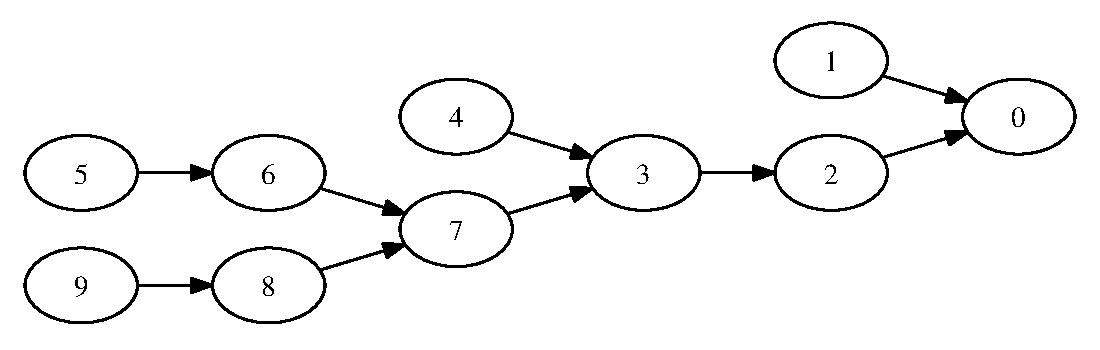
\includegraphics[scale=0.6]{figures/topo.eps}
\caption{汇聚树节点拓扑结构}\label{collection-tree}
\end{figure}

\subsubsection{CTP协议性能评价}
评价CTP协议的性能主要根据3个指标:开销,平均深度和包投递率。

{\kai 开销}是指平均每个单播包传输的总次数。由于包传输对节点来说所消耗的能量是相当可观的,因此开销的大小将直接影响到网络的生存时间,开销越大,网络的生存时间越短。它与路径的跳数,每个连接的重传数以及由于包丢失而造成的浪费有关。

{\kai 平均深度}指的是汇聚树的平均深度。如果所有的连接是完好的,没有重传和丢包,那么平均深度将是开销的下界。两者间的差异意味着选择连接的质量,这可能是由于重传或丢包所造成的,高效的路由算法可以使这个差异最小化。

{\kai 投递率}是指根节点收到的不重复消息的百分率,即根节点收到的数据包中除去重复的包所剩余的包数与所有节点发出的本地数据包数之比。这个指标的大小可以体现出丢包数,投递率越高说明丢包数越少。

在仿真结果中,可以通过监视节点转发引擎中的转发事件(包括了本地发送的包),计算出本地包的个数和转发次数。平均开销计算公式如下:
\begin{equation}
\text{\kai 平均开销} = \frac{\text{\kai 本地包发送次数} + \text{\kai 转发包发送次数}}{\text{\kai 本地包个数}}
\end{equation}
平均深度的计算就需要先获知汇聚树的拓扑结构,这可以通过监视父节点选择的变化获得。投递率的计算除了要监视转发事件之外,还需要监视根节点的包接收事件以得到投递成功的信息。根据上述方法对10个节点进行仿真,对比了使用标准LE和4BITLE的两种情况,得到表\ref{sim-result}所示结果:
\vspace{-5pt}
\begin{table}[ht]
\centering
\caption{\hei 仿真结果}\label{sim-result}
\vspace{5pt}
\wuhao
\begin{tabular}{l|rrr}
		& ~~~~~~~~标准LE& ~~~~~~~~4BITLE &增大消息缓存的4BITLE \\
\hline
转发包发送次数	&	3294 & 3002 & 3326 \\
本地包发送次数	&	1292 & 1272 & 1205 \\
本地包总个数	& 	121 & 120 & 124 \\
投递包个数(有重复)&	252 & 334 & 123 \\
投递包个数(去重复)&	109 & 115 & 117 \\
开销		&	37.90 & 35.62  & 36.54 \\
本均深度	&	2.0 & 2.9 & 3.5 \\
投递率		&	90.08\% & 95.83\% & 94.35 \\
\end{tabular}
\end{table}

从结果中可以看出,包发送的次数几乎是根节点实际接收到的包数的20$\sim$40倍,这是由于仿真使用的节点间连接质量(见表\ref{nodes-link-quality})设定的较差,导致节点间不断发生重传所造成的,这也是开销比平均深度大10$\sim$20倍左右的原因。但即便是在通信质量如此差的网络中,CTP协议还是可以成功地建立起多跳汇聚树,并保持了在90\%以上的较高的投递率,说明CTP协议是比较可靠的。

对比标准LE和4BITLE的数据可以发现,4BITLE即使在本均深度不如标准LE的情况下投递率还是明显高于标准LE的投递率,这是由于4BITLE使用了各层的信息得出的估计值比标准LE更精确,从而选择质量较差的连接的概率较小,丢包数也相应地减小。比较有重复的投递包个数和去重复的投递包个数可以发现,增大消息缓存后的4BILTE的包重复数(6个)远小于原来的4BITLE(219个),这是由于消息缓存的增大使节点存储已收到的包数增加,在缓存中停留的时间增长,从而发现重复包的概率增大。

\section{部署}
\subsection{自主开发节点简介}
实际部署的节点使用的是自主开发的npumote平台节点,它使用微处理器Atmega1281和无线模块RF230,配备了温湿度、光照等传感器,主要用于温室群的精准农业监控。

\subsection{为TinyOS 2.x添加平台支持}
由于TinyOS 2.x并没有直接支持我们的平台npumote,因而要对它做一些修改。主要的修改有如下几个方面:
\vspace{-10pt}
\begin{enumerate}
	\item{修改make系统:} 增加对avrisp2烧写器支持;增加npumote编译目标规则。
	\item{修改硬件参数和连接方式:} 修改串口的收发波特率;将AM层直接接到UniqueLayerC模块而不通过IEEE154网络层;增加EEPROM模块;修改RF230信道使程序在编译时可以通过增加RF230\_DEF\_CHANNEL标记设定信道值从EEPROM中读取;
\end{enumerate}
\vspace{-10pt}
将所有的改动以GNU diff格式记录到文件\texttt{npumote.patch}。在unix环境中,使用者只须将\texttt{npumote.patch}放在\texttt{tinyos-2.x}同一个目录下,进入\texttt{tinyos-2.x}目录, 执行命令:
\begin{lstlisting}[language=bash,numbers=none]
    patch -p1 <../npumote.patch
\end{lstlisting}
即可使TinyOS 2.x支持npumote平台。

\subsection{将程序烧写到节点中}
在使用CTP协议的应用程序源代码目录\texttt{apps/tests/TestNetwork}下运行以下命令将编译生成二进制文件并烧写到节点中:
\begin{lstlisting}[language=bash,numbers=none]
    make npumote install.<`节点号`> avrisp2,<`烧写器端口`>
\end{lstlisting}
如果编译通过但烧写失败,则需要检查烧写器端口是否书写正确并且确认当前用户是否具有该端口的读写权限。

\subsection{节点中程序的调试}
由于节点的资源有限,程序的调试相对比较困难。传统的做法是使用节点上的3个LED灯提供节点的状态信息。比如在节点启动完毕事件触发时,在程序中指定将红色的LED灯开启;在接收或发送消息时,使LED灯闪烁等方法得知节点的工作信息。这种方法是最实时有效的,但也是原始和效率低下的。TinyOS 2.x支持printf库的方法可通过串口向PC机发送调试信息,使调试方便了不少,但仍存在诸多限制,如在串口开启之前的调试信息无法发送,不能设置断点和查看更改寄存器信息,修改程序后要重新烧写节点等问题。另外,节点也可以使用JTAG硬件调试器调试,由于我们自主开发节点对这种方法的工具链支持还不完全,故不在此详述。总之,节点中程序的调试还有许多工作可以做,
可以作为以后研究工作的重点。

\subsection{节点部署}
节点号为0的节点在该应用程序中作为根节点使用,把它通过串口与上位机相连以便接收并处理汇聚上来的数据。其它节点的部署方法详见“无线传感器网络部署及其覆盖问题研究”\ucite{liuliping2006}。
